% Chapter 3

\chapter{Algorithms for Automatic Bug Triaging}
The various algorithms for Automatic Bug Triaging depend on the dataset being used. The training dataset obtained after parsing, has been subjected to stop-word removal and stemming. Snowball Stemming algorithm is used for stop-word removal and stemming. Multinomial NB classifier is used for converting the data set to feature vectors. 

%\section{Algorithm}
The product, component and short description of each bug from the Training data set are parsed using a XSLT parser to obtain an unified text file. The report ID of each bug from the \texttt{assigned-to.xml} file is taken and the "when" attribute of each update of the bug is taken and matched with the corresponding entries in \texttt{short-desc.xml}, \texttt{product.xml} and \texttt{component.xml} and extracted and output to a text file in a format suitable for text processing.




\section{Snowball Stemming Algorithm}
The above parsed data has to be processed to extract the keywords. Stop-word and special Characters removal is first performed using the Natural Language ToolKit in python. Then the same Toolkit is used to perform stemming on the text after the stop-words are removed. 

\begin{algorithm}[H]
	\DontPrintSemicolon % Some LaTeX compilers require you to use \dontprintsemicolon instead
	\SetKwFunction{STEM}{STEM}
	\KwIn{$F$: Text file containing the Training dataset
	\newline $S$: Set of stop-words for the language English}
	\KwOut{$FP$ : Text file containing the Training dataset after stop-word removal and Stemming}
	\ForEach(\tcp*[h]{For each line in the file}){ line $L$ in $F$} { 
		\ForEach(\tcp*[h]{For each word in the line}){ word $W$ in $L$}{
			\If(\tcp*[h]{If the word is not a stop-word}){$W$ not in  $S$} {
		\STEM{$W$} \;
	}
	\tcc{Performs Stop-word removal and Stemming on each $W$}
		}
	
	}
	\Return{$FP$}\;
	\caption{{\sc Snowball Stemming} - Removes Stop-words and performs Stemming}
	\label{algo:Snowball Stemming}
\end{algorithm}

\section{Naive Bayes Text Classifier Algorithm}
Through supervised learning the system learns from the TDS(Training data set)- the keywords present in the description of the bug and the developer to whom it was assigned. It also gathers information about the reassignment of bugs.

The system uses Naive Bayes classifier to classify the new bugs reported, to calculate the probability of it being assigned to a developer. Naive Bayes is a probabilistic technique that uses Bayes rule of conditional probability to determine the probability that an instance belongs to a certain class. Bayes rules states that, "The probability of a class conditioned on an observation to the prior probability of the class times the probability of the observation conditioned on the class" and can be denoted as follows:

\[{P(Class|Observation)} = {\frac{P(Observation|Class)*P(Class)}{P(Observation)}}\]

For example, if the word 'concurrency' occurs more frequently in the reports resolved by developer A than in the reports resolved by developer B, the classifier would predict A as a potential fixer for a new bug report containing the word 'concurrency'. “ Naive Bayes ” is so called because it makes the strong assumption that features are independent of each other, given the label (the developer who resolved the bug).

\begin{algorithm}[H]
	\DontPrintSemicolon % Some LaTeX compilers require you to use \dontprintsemicolon instead
	\SetKwFunction{STEM}{STEM}
	\KwIn{$T$: Training corpus
	\newline $B$: New Bug Report}
	\KwOut{$d_j$ : The developer with the highest probability to whom the bug will be assigned.}
	$From\ Training\ corpus,\ extract\ Vocabulary$ \;
	\ForEach(\tcp*[h]{Calculate P($d_j$) terms}){ developer $d_j$ in $D$} { 
		$reports_j \gets {all\ bug\ reports\ in\ developer\ d_j}$ \;
		$P(d_j) \gets {\frac{|reports_j|}{|total\ no.\ reports|}}$ \;
	
	}
	$Text_j \gets {single\ text\ containing\ all\ reports_j}$ \;
\ForEach(\tcp*[h]{Calculate P($w_k | d_j$)  terms}){ word $w_k$ in $Vocabulary$} { 
		$n_k \gets {no.\ of\ occurences\ of\ w_k\ in\ Text_j}$ \;
		$P(w_k |d_j) \gets {\frac{n_k+const}{n+const|Vocabulary|}}$ \;
		
		\tcc{ $const = 1$, Laplacian Smoothing constant}
	
	}	
	
	\Return{$d_j\ with\ highest\ probability$}\;
	\caption{{\sc Naive Bayes Classifier} - Text classification}
	\label{algo:Naive Bayes}
\end{algorithm}

\section{Multinomial Naive Bayes Algorithm}
Feature Vector :
		$W$=($w_1$, $w_2$, $w_3$, ..., $w_n$)
\begin{equation}
	log\ p(D_k|W) = log\ p(D_k) + \sum\limits^{N}_{i=1}w_i\ .\ log\ p(w_i|D_k)
\end{equation}
Prior : ${\frac{|N_c|}{|N|} }$
Conditional Probability : $\frac{count(w,D_k)+1}{count(D_k)+|V|}$		
\begin{algorithm}[H]
	\DontPrintSemicolon % Some LaTeX compilers require you to use \dontprintsemicolon instead
	\SetKwFunction{STEM}{STEM}
	\KwIn{$R$: Training Corpus(List of bug reports)
	\newline $C$: List of developers}
	\KwOut{V-vocabulary,prior and condprob }
	$V \gets {\ extract\ Vocabulary}$ \;
    $N \gets {\ count\ bug\ Reports}$ \;

   
	\ForEach{ developer $d$ in $D$} 
	{     
		$N_c \gets {\ count\ bug\ reports\ in\ developer\ d\ from\ R}$ \;
    		$prior(d) \gets {\frac{|N_c|}{|N|} }$ \;
    		$words_c \gets {\ collect\ all\ words\ from\ all\ bug\ reports\ in\ developer\ c}$ \;	
    	
    		\ForEach{ word $w$ in $V$} 
    		{
    			$T_c \gets {\ count\ occurences\ of\ word(w,words_c)}$ \;
    			$T_c' \gets {\ count words(c)}$ \;
    			$condprob(w|c) \gets {\frac{|T_c+1|}{T_c' + 1 } }$ \;
    		} 
	}
	\Return{$V\ ,prior\ and\ condprob$}\;
	\caption{{\sc Train MultinomialNB} - Text classification}
	\label{algo:Train MNB}
\end{algorithm}
\newpage
\begin{algorithm}[H]
	\DontPrintSemicolon % Some LaTeX compilers require you to use \dontprintsemicolon instead
	\SetKwFunction{STEM}{STEM}
	\KwIn{$C$: List of Developers
	\newline $V$: Vocabulary
	\newline prior
	\newline condprob
	\newline $R$: Bug Report}
	\KwOut{$d$: The developer with the highest probability to whom the bug maybe assigned to.}
	$W \gets {\ extract\ words from\ Report\ R}$ \;
	\ForEach{ developer $d$ in $D$} 
	{     
    		$P(d|R) \gets {log(prior(d))}$ \;
    		\ForEach{ word $w$ in $W$} 
    		{
    			freq = count(w,R) \;
    			$P(d|R)$ += freq * log(condprob($w|d$))
	    	}
    }
	
	\Return{$argmax_d\ P(d|R)$}\;
	\caption{{\sc Apply MultinomialNB} - Text classification}
	\label{algo:Apply MNB}
\end{algorithm}

\section{Tf- idf Weight Calculation}
 Term Frequency - Inverse Document Frequency(tf-idf) is a numerical statistic that is intended to reflect how important is a word to a document in a collection or corpus. This is to minimize the frequently occurring words in all the documents(bug reports) from reducing the efficiency in bug assignment. 
\[{tf(t,doc) = 0.5 + \frac{0.5 \times f(t, doc)}{\max\{f(w, doc):w \in doc\}} }\] 
\[{ idf(t, DOC) = \log \frac{N}{1+|\{doc \in DOC: t \in doc\}|}  }\]
\[{ tfidf(t,doc,DOC) = tf(t,doc) \times idf(t, DOC)  }\]

\section{Linear Support Vector Machine}
An Support Vector Machine (SVM) is a kind of large margin classifier. It is a vector space based Machine Learning method, where the goal is to find a decision boundary between two or more classes that is maximally far from any point in the training data. An Binary SVM model is a representation of the examples as points in space, mapped so that the examples of the separate categories are divided by a clear gap that is as wide as possible.
\[{D = \left\{ (x_i, y_i)\mid x_i \in {R}^p,\, y_i \in \{ -1,1\}\right\}_{i=1}^n}\]
Multi-class SVM is implemented by reducing the single multi-class problem into multiple binary classification problems.(one-versus-all).

\section{Folding}
In folding based training and validation approach, also known as cross validation, the algorithm first collects all bug reports to be used for TDS (Training Data Set) sorts them in chronological order(based on the update time of the bug) and then divides them into \textit{n} folds. In the first run, fold 1 is used to train the classifier and then to predict the VDS (Verified Data Set). In the second run, fold 2 bug reports are added to TDS. In general, after validating the VDS from fold \textit{n}, VDS is added to the TDS for validating fold \textit{n+1}. For example, we chose \textit{n=10} and carried out 9 iterations of the validation process using incremental learning.
\newpage
%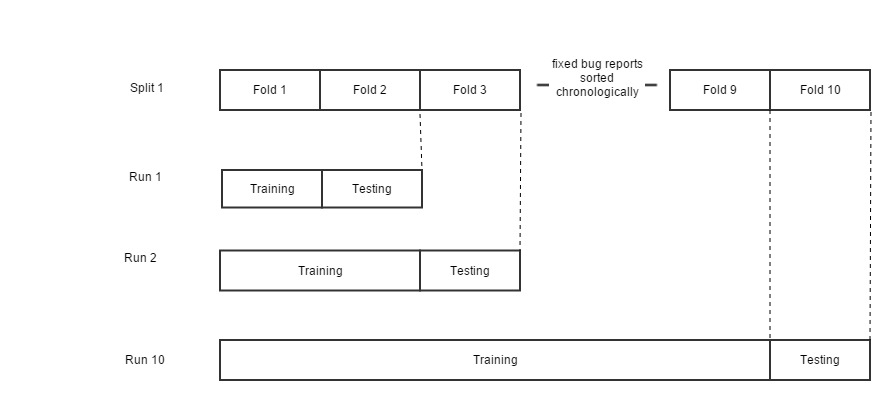
\includegraphics[height=15cm,width=15cm]{folding}
\begin{figure}[hbt]
\begin{center}

\includepdf[scale=0.8,pages={27}, offset =75 -75]{review3_v3.pdf}
\caption{FOLDING}
\end{center}
\end{figure}
\newpage

\section{Goal oriented tossing graph}
When a bug is assigned to a developer for the first time and if she is unable to fix it, the bug is assigned(tossed) to another developer. Thus a bug is tossed from one developer to another until a developer is eventually able to fix it. Based on these tossing path, goal oriented tossing graphs were proposed. Tossing graphs are weighted directed graphs such that each node represents a developer, and each directed edge from D1 to D2 represents the fact that bug is assigned to developer D1 was tossed and eventually fixed by developer D2. The weight of the edge between two developers is the probability of a toss between them, based on bug tossing history. We denote a tossing event from developer D to $D_j  as D \implies D_j$.

\newpage
\begin{table}[hbt]
\begin{center}

\includepdf[scale=0.8,pages={31}, offset =75 -75]{review3_v3.pdf}
\caption{GOAL ORIENTED TOSSING GRAPH}
\end{center}
\end{table} 

\newpage
\section{Prediction Accuracy}

If the first developer in our prediction list matches the actual developer who fixed the bug, we have a hit for the Top 1 developer count. Similarly, if the second developer in our prediction list matches the actual developer who fixed the bug, we have a hit for the Top 2 developer count. For example, if there are 100 bugs in the VDS and for 20 of those bugs the actual developer is the first developer in our prediction list, the prediction accuracy for Top 1 is 20\%; similarly, if the actual developer is in our Top 2 for
60 bugs, the Top 2 prediction accuracy is 60\%.
